% Generated by book/tools/notebook_to_tex.py. Do not edit by hand.

\chapter[BERT 회귀 분석 (Regression \& Trainer)]{BERT 회귀 분석 (Regression \& Trainer)}

\label{ch:09}

\markboth{BERT 회귀 분석 (Regression \& Trainer)}{BERT 회귀 분석 (Regression \& Trainer)}

\chaptermeta{09_bert_regression/09_bert_regression.ipynb}{https://colab.research.google.com/github/yoon-gu/neuqes-101/blob/master/09_bert_regression/09_bert_regression.ipynb}{DistilBERT 파인튜닝과 Trainer의 첫 사용}



\index{1BERT regression@BERT regression}

\index{1DistilBERT@DistilBERT}

\index{1Trainer@Trainer}

\index{1TrainingArguments@TrainingArguments}

\index{1problem type@problem\_type}

\index{1regression@regression}

\index{1MSELoss@MSELoss}

\index{1fp16@fp16}

\index{1Adam@Adam}

\index{1compute metrics@compute\_metrics}

\index{1fine tuning@fine-tuning}

\index{0파인튜닝@파인튜닝}

\index{0트레이너@트레이너}

\index{0학습 인자@학습 인자}

\index{0회귀 헤드@회귀 헤드}

\index{0평균제곱오차@평균제곱오차}

\index{0혼합 정밀도@혼합 정밀도}

\index{0GPU 메모리@GPU 메모리}

\index{1AutoModelForSequenceClassification@AutoModelForSequenceClassification}

\index{1num labels 1@num\_labels=1}

\index{1problem type regression@problem\_type="regression"}

\index{1evaluation strategy@evaluation\_strategy}

\index{1save strategy@save\_strategy}

\index{1learning rate@learning\_rate}

\index{1per device train batch size@per\_device\_train\_batch\_size}

\index{1weight decay@weight\_decay}

\index{1VRAM@VRAM}

\index{1nvidia smi@nvidia-smi}

\index{0정규방정식@정규방정식}

\index{0경사하강법@경사하강법}

\index{0학습률@학습률}

\index{0배치 크기@배치 크기}

\index{0가중치 감쇠@가중치 감쇠}



\section{변화추적표}

\begin{booktable}{9장 변화추적표}{tab:ch09-01}
\begin{adjustbox}{max width=\textwidth}
\begin{tabular}{@{}lllllll@{}}
\toprule
Ch & 모델 & 토크나이저 & 데이터 & Output Head & Activation & Loss \\
\midrule

2 & \inlinecode{LinearRegression()} & \inlinecode{TfidfVectorizer()} & Yelp (별점 1-5) & (1차원) & 없음 & \inlinecode{MSELoss} \\
7-8 & DistilBERT (추론·데이터 파이프라인) & \inlinecode{AutoTokenizer.from\_pretrained(...)} & Yelp / 영어 예시 & 사전학습 헤드 & softmax & --- \\
\textbf{9 ← 여기} & \textbf{DistilBERT 파인튜닝} & \inlinecode{AutoTokenizer.from\_pretrained(...)} & Yelp (별점 1-5, \ref{ch:02}장과 동일) & \textbf{\inlinecode{Linear(H,\ 1)}} & 없음 & \textbf{\inlinecode{MSELoss}} \\
\bottomrule
\end{tabular}
\end{adjustbox}
\end{booktable}

전체 20장 표는 \href{https://github.com/yoon-gu/neuqes-101\#챕터별-변화추적표}{루트 README.md}를 참고하세요.



\section{변경점: \ref{ch:08}장 대비}

\begin{booktable}{9장 변경점 요약}{tab:ch09-02}
\begin{adjustbox}{max width=\textwidth}
\begin{tabular}{@{}lll@{}}
\toprule
축 & \ref{ch:08}장 & \ref{ch:09}장 \\
\midrule

모델 & 모델 로드 없음 & \textbf{\inlinecode{AutoModelForSequenceClassification} (\inlinecode{num\_labels=1}, \inlinecode{problem\_type="regression"})} \\
학습 & 없음 & \textbf{있음} --- Trainer.train() \\
Loss & --- & \textbf{\inlinecode{MSELoss}} (\ref{ch:02}장과 같은 식, 최소화 방식만 SGD로 바뀜) \\
데이터 & Yelp 토크나이저 옵션 실험 & Yelp 4,000 학습 + 1,000 평가 (별점 1-5 float 라벨) \\
GPU & 옵션 & \textbf{필수} --- fp16, 옵티마이저+gradient가 VRAM에 추가 \\
작업 시간 & 즉시 & \textbf{수 분} (T4에서 \textasciitilde5-8분 학습) \\
\bottomrule
\end{tabular}
\end{adjustbox}
\end{booktable}

\textbf{핵심 변화}: 같은 MSELoss이지만 \emph{어떻게 최소화하느냐} 가 다릅니다.

\begin{itemize}
\tightlist
\item
  \ref{ch:02}장 \inlinecode{LinearRegression}: 정규방정식으로 \emph{한 번에} 닫힌 해 도출. 1초 미만.
\item
  \ref{ch:09}장 BERT: SGD/Adam으로 \emph{수천 번 step} 을 밟으며 점진적 최소화. fp16, 옵티마이저 모멘텀, gradient accumulation 등 도구가 한꺼번에 등장.
\end{itemize}

\ref{ch:06}장 끝의 “sklearn vs HuggingFace 미리보기” 표가 이 장에서 실제 코드로 펼쳐집니다.



\section{\texorpdfstring{손실 노트}{손실 노트}}

수식은 \ref{ch:02}장과 동일합니다.

\begin{equation}
\label{eq:ch09-01}
L = \frac{1}{N} \sum_{i=1}^{N} (y_i - \hat y_i)^2
\end{equation}

식~\eqref{eq:ch09-01}은 회귀에서 사용하는 Mean Squared Error의 정의입니다.

다른 점은 \emph{어떻게 이 \(L\)을 최소화하느냐} 입니다.

\begin{booktable}{9장 손실 노트 표}{tab:ch09-03}
\begin{adjustbox}{max width=\textwidth}
\begin{tabular}{@{}lll@{}}
\toprule
측면 & \ref{ch:02}장 (\inlinecode{LinearRegression}) & \ref{ch:09}장 (BERT) \\
\midrule

최소화 방법 & 정규방정식 \(w = (X^\top X)^{-1} X^\top y\) --- 한 번에 닫힌 해 & Adam optimizer --- gradient descent step을 수천 번 \\
학습 시간 & 1초 미만 & T4에서 5-8분 \\
결정성 & 입력이 같으면 가중치가 정확히 같음 & random seed·batch 순서에 따라 매번 미세 차이 \\
왜 BERT를 쓰나 & 단어 독립 가정의 한계 (\inlinecode{"not\ bad"} ≠ \inlinecode{"bad"} 구분 불가) & 문맥을 attention으로 학습해 더 정확한 회귀 \\
\bottomrule
\end{tabular}
\end{adjustbox}
\end{booktable}

Hugging Face \inlinecode{Trainer} 는 \inlinecode{problem\_type="regression"} 을 보고 자동으로 \inlinecode{MSELoss} 를 적용합니다. 우리가 직접 \inlinecode{criterion\ =\ nn.MSELoss()} 같은 코드를 쓸 필요가 없습니다.



\section{토크나이저 노트}

\ref{ch:07}·\ref{ch:08}장과 동일한 \inlinecode{distilbert-base-uncased} WordPiece 토크나이저를 그대로 사용합니다. 이 장는 모델·loss·학습 루프에 집중하므로 토크나이저 파이프라인은 \ref{ch:08}장에서 익힌 그대로 (\inlinecode{map(batched=True)} + \inlinecode{DataCollatorWithPadding}).

\begin{previewBox}{미리보기}
\textbf{다음 장(\ref{ch:10}·\ref{ch:11}장)}: 같은 토크나이저, 같은 데이터지만 task가 binary 분류로 바뀝니다. \ref{ch:10}장에서 sigmoid+BCE 방식, \ref{ch:11}장에서 softmax+CE 방식을 \emph{별도 학습} 해 두 방식을 비교합니다.
\end{previewBox}



\Needspace{5\baselineskip}
\begin{lstlisting}
!pip install -q transformers datasets
\end{lstlisting}

\begin{codeRead}
\textbf{1행}의 \inlinecode{!pip install -q transform...}에서는 Colab 실행에 필요한 패키지를 설치합니다.
\end{codeRead}



\Needspace{11\baselineskip}
\begin{lstlisting}
import warnings
warnings.filterwarnings("ignore")

import numpy as np
import pandas as pd
import matplotlib.pyplot as plt
import seaborn as sns
import torch
from datasets import load_dataset
from transformers import (
    AutoTokenizer, AutoModelForSequenceClassification,
    Trainer, TrainingArguments,
)
from sklearn.metrics import mean_squared_error, mean_absolute_error, r2_score

plt.rcParams["axes.unicode_minus"] = False
\end{lstlisting}

\noindent\emph{앞 블록은 필요한 라이브러리와 기본 설정을 준비하는 단계입니다. 이어지는 블록에서는 앞에서 만든 중간 값을 다음 계산으로 넘기는 단계로 넘어갑니다.}

\Needspace{11\baselineskip}
\begin{lstlisting}[firstnumber=18]
print(f"PyTorch:        {torch.__version__}")
print(f"CUDA available: {torch.cuda.is_available()}")
if torch.cuda.is_available():
    print(
        f"GPU:             "
        f"{torch.cuda.get_device_name(0)}"
    )
else:
    print(
        "Warning: CPU runtime — training will be very "
        "slow. Switch to T4 recommended."
    )
\end{lstlisting}

\noindent\textbf{출력 형태.}
\begin{lstlisting}[style=bookoutput]
PyTorch:        2.x.x
CUDA available: True
GPU:            Tesla T4
\end{lstlisting}
\par\vspace{0.9em}

\begin{codeRead}
\inlinecode{numpy, pandas, matplotlib, PyTorch, datasets} 같은 주요 패키지를 불러옵니다.
\end{codeRead}



\textbf{baseline VRAM} --- 모델 로드 전:



\Needspace{5\baselineskip}
\begin{lstlisting}
!nvidia-smi
\end{lstlisting}

\begin{codeRead}
\textbf{1행}의 \inlinecode{!nvidia-smi}에서는 앞 단계에서 만든 값을 바탕으로 다음 계산을 수행합니다.
\end{codeRead}



\section{데이터 준비}

\ref{ch:08}장에서 익힌 \inlinecode{datasets} + 토크나이저 패턴을 그대로 적용합니다. 차이는 라벨을 \emph{float} 형으로 바꾼다는 점입니다 --- 회귀이므로 정답이 정수 클래스가 아닌 실수입니다.

별점 1-5를 그대로 학습 라벨로 사용합니다 (\inlinecode{label} 필드는 0-4로 저장돼 있어 +1).



\Needspace{11\baselineskip}
\begin{lstlisting}
tokenizer = AutoTokenizer.from_pretrained("distilbert-base-uncased")

ds = load_dataset("yelp_review_full")

train_ds = ds["train"].shuffle(seed=42).select(range(4000))
eval_ds  = ds["test"].shuffle(seed=42).select(range(1000))

def tokenize_fn(batch):
    out = tokenizer(
        batch["text"],
        truncation=True,
        max_length=128,
    )

    out["labels"] = [float(lbl) + 1.0 for lbl in batch["label"]]
    return out
\end{lstlisting}

\noindent\emph{앞 블록은 데이터를 불러오고 학습에 맞는 형태로 정리하는 단계입니다. 이어지는 블록에서는 텍스트를 모델 입력 텐서로 바꾸는 단계로 넘어갑니다.}

\Needspace{11\baselineskip}
\begin{lstlisting}[firstnumber=18]
train_tok = train_ds.map(
    tokenize_fn,
    batched=True).remove_columns(["text", "label"],
)
eval_tok  = eval_ds.map(
    tokenize_fn,
    batched=True).remove_columns(["text", "label"],
)

print(train_tok)
print(
    f"\nFirst sample label: "
    f"{train_tok[0]['labels']}  (float)"
)
\end{lstlisting}

\noindent\textbf{출력 형태.}
\begin{lstlisting}[style=bookoutput]
Dataset({
  features: [...],
  num_rows: ...
})
\end{lstlisting}
\par\vspace{0.9em}



\section{\texorpdfstring{모델 로드}{모델 로드}}

\ref{ch:07}장에서는 사전학습된 분류 헤드(\inlinecode{distilbert-base-uncased-finetuned-sst-2-english}, num\_labels=2)를 그대로 썼습니다. 이번엔 본체 모델만 받고 \textbf{분류 헤드를 새로} 만듭니다 --- \inlinecode{num\_labels=1} 이라 출력 차원이 1, \inlinecode{problem\_type="regression"} 이라 \inlinecode{Trainer} 가 자동으로 MSELoss 사용.



\Needspace{11\baselineskip}
\begin{lstlisting}
model = AutoModelForSequenceClassification.from_pretrained(
    "distilbert-base-uncased",
    num_labels=1,
    problem_type="regression",
)
print(
    f"Parameters:    "
    f"{sum(p.numel() for p in model.parameters()):,}"
)
print(f"Classifier:    {model.classifier}")
print(f"problem_type:  {model.config.problem_type}")
\end{lstlisting}

\noindent\textbf{출력 형태.}
\begin{lstlisting}[style=bookoutput]
Total parameters:     ...
Trainable parameters: ...
Classifier:           ...
\end{lstlisting}
\par\vspace{0.9em}



\textbf{경고 메시지를 보셨을 겁니다} --- \inlinecode{Some\ weights\ of\ DistilBertForSequenceClassification\ were\ not\ initialized\ ...}. 분류 헤드(\inlinecode{Linear(768,\ 1)})가 새로 만들어지면서 \emph{랜덤 초기화} 됐다는 알림입니다. 이 부분이 학습으로 채워지고, BERT 본체는 사전학습 가중치를 미세 조정합니다 (transfer learning의 본 모습).

\subsection{학습 파라미터}

\inlinecode{from\_pretrained()} 직후엔 \emph{모든} 파라미터가 학습 대상입니다 (\inlinecode{requires\_grad=True}). 그러나 데이터가 작거나 빠른 학습이 필요하면 BERT 본체를 \emph{동결(freeze)} 하고 분류 헤드만 학습하기도 합니다. 학습 시작 전에 \emph{전체 vs 학습되는 파라미터} 를 한 번 확인하는 게 좋은 습관입니다.



\Needspace{11\baselineskip}
\begin{lstlisting}
def param_summary(m):
    total     = sum(p.numel() for p in m.parameters())
    trainable = sum(p.numel() for p in m.parameters() if p.requires_grad)
    frozen    = total - trainable
    return total, trainable, frozen

total, trainable, frozen = param_summary(model)
print(
    f"Total parameters:     {total:>13,}  ("
    f"{total/1e6:.1f} M)"
)
print(
    f"Trainable parameters: {trainable:>13,}  ({trainable/1e6:.1f} M, "
    f"{trainable/total:.1%})"
)
print(
\end{lstlisting}

\noindent\textbf{출력 형태.}
\begin{lstlisting}[style=bookoutput]
Total parameters:     ...
Trainable parameters: ...
Classifier:           ...
\end{lstlisting}
\par\vspace{0.9em}

\noindent\emph{앞뒤 블록은 모두 앞에서 만든 중간 값을 다음 계산으로 넘기는 단계입니다. 길이를 나누어 같은 흐름을 단계별로 확인합니다.}

\Needspace{6\baselineskip}
\begin{lstlisting}[firstnumber=17]
    f"Frozen parameters:    {frozen:>13,}  ({frozen/1e6:.1f} M, "
    f"{frozen/total:.1%})"
)
print(f"\nDefault — all layers are trainable")
\end{lstlisting}

\noindent\textbf{출력 형태.}
\begin{lstlisting}[style=bookoutput]
Total parameters:     ...
Trainable parameters: ...
Classifier:           ...
\end{lstlisting}
\par\vspace{0.9em}



\subsection{BERT 본체 동결}

본 학습은 \emph{모든 파라미터} 를 학습하지만, 동결 패턴이 어떻게 적용되는지 \emph{별도 모델 인스턴스} 로 한 번 보여드립니다 (이 시연 모델은 학습에 사용하지 않습니다).



\Needspace{11\baselineskip}
\begin{lstlisting}
demo_model = AutoModelForSequenceClassification.from_pretrained(
    "distilbert-base-uncased", num_labels=1, problem_type="regression",
)

for p in demo_model.distilbert.parameters():
    p.requires_grad = False

t, tr, fr = param_summary(demo_model)
print(f"After freezing BERT body:")
print(f"  Total:       {t:>13,}")
print(
    f"  Trainable:   {tr:>13,}  ("
    f"{tr/t:.1%})  ← classification head only"
)
print(
    f"  Frozen:      {fr:>13,}  ("
\end{lstlisting}

\noindent\textbf{출력 형태.}
\begin{lstlisting}[style=bookoutput]
Total parameters:     ...
Trainable parameters: ...
Classifier:           ...
\end{lstlisting}
\par\vspace{0.9em}

\noindent\emph{앞뒤 블록은 모두 앞에서 만든 중간 값을 다음 계산으로 넘기는 단계입니다. 길이를 나누어 같은 흐름을 단계별로 확인합니다.}

\Needspace{10\baselineskip}
\begin{lstlisting}[firstnumber=17]
    f"{fr/t:.1%})  ← BERT body"
)
print(
    f"\nOnly "
    f"{tr:,} classification head parameters update — fast, low memory."
)
print(
    f"Tradeoff: BERT body cannot adapt to the task — "
\end{lstlisting}

\noindent\textbf{출력 형태.}
\begin{lstlisting}[style=bookoutput]
Total parameters:     ...
Trainable parameters: ...
Classifier:           ...
\end{lstlisting}
\par\vspace{0.9em}

\noindent\emph{앞 블록은 앞에서 만든 중간 값을 다음 계산으로 넘기는 단계입니다. 이어지는 블록에서는 필요한 라이브러리와 기본 설정을 준비하는 단계로 넘어갑니다.}

\Needspace{11\baselineskip}
\begin{lstlisting}[firstnumber=25]
    f"usually train the body too if data is sufficient."
)
print(
    f"\n(This demo model is not used for the actual "
    f"training — del demo_model frees memory.)"
)

import gc
del demo_model
gc.collect()
if torch.cuda.is_available():
    torch.cuda.empty_cache()
\end{lstlisting}

\noindent\textbf{출력 형태.}
\begin{lstlisting}[style=bookoutput]
PyTorch:        2.x.x
CUDA available: True
GPU:            Tesla T4
\end{lstlisting}
\par\vspace{0.9em}



\textbf{언제 동결을 쓰나}

\begin{itemize}
\tightlist
\item
  \textbf{분류 헤드만 학습 (모든 본체 동결)}: 데이터 매우 작음 (수백 건), 빠른 baseline 필요.
\item
  \textbf{하위 N개 layer 동결}: 일반 언어 표현은 BERT 그대로, 상위 layer만 task 적응.
\item
  \textbf{모든 파라미터 학습 (default)}: 데이터 충분 (수천 건+), 본체도 task에 맞게 적응.
\end{itemize}

이 장는 4,000건이라 default(전체 학습)이 가장 좋은 선택입니다.



\Needspace{5\baselineskip}
\begin{lstlisting}
!nvidia-smi
\end{lstlisting}



모델 가중치(\textasciitilde67M 파라미터, fp32 \textasciitilde255 MB)가 GPU에 올라간 상태입니다. 학습이 시작되면 \emph{옵티마이저 모멘텀(2배) + gradient(1배)} 가 추가되어 VRAM이 더 늘어납니다.



\section{\texorpdfstring{Trainer 설정}{Trainer 설정}}

\ref{ch:06}장 끝에서 미리 본 코드 형태가 이제 실제로 등장합니다. \inlinecode{TrainingArguments} 한 객체에 학습 하이퍼파라미터를 모두 모으고, \inlinecode{Trainer} 가 학습 루프·평가·로그·체크포인트를 자동화합니다.



\Needspace{11\baselineskip}
\begin{lstlisting}
training_args = TrainingArguments(
    output_dir="./ch09_output",
    num_train_epochs=2,
    per_device_train_batch_size=16,
    per_device_eval_batch_size=32,
    learning_rate=2e-5,
    fp16=True,
    eval_strategy="epoch",
    logging_steps=50,
    save_strategy="no",
    report_to="none",
    seed=42,
)

\end{lstlisting}

\noindent\emph{앞 블록은 학습 설정을 만들고 학습 루프를 실행하는 단계입니다. 이어지는 블록에서는 앞에서 만든 중간 값을 다음 계산으로 넘기는 단계로 넘어갑니다.}

\Needspace{6\baselineskip}
\begin{lstlisting}[firstnumber=15]
print(
    f"Total training steps: "
    f"{len(train_tok) // training_args.per_device_train_batch_size * training_args.num_train_epochs}"
)
\end{lstlisting}

\noindent\textbf{출력 형태.}
\begin{lstlisting}[style=bookoutput]
Output varies by runtime, seed, and sampled data.
Running the cell in Colab prints the corresponding string or table.
\end{lstlisting}
\par\vspace{0.9em}



\Needspace{10\baselineskip}
\begin{lstlisting}
def compute_metrics(eval_pred):
    preds, labels = eval_pred
    preds = preds.flatten()
    return {
        "mse": float(mean_squared_error(labels, preds)),
        "mae": float(mean_absolute_error(labels, preds)),
        "r2":  float(r2_score(labels, preds)),
    }
\end{lstlisting}



\Needspace{11\baselineskip}
\begin{lstlisting}
trainer = Trainer(
    model=model,
    args=training_args,
    train_dataset=train_tok,
    eval_dataset=eval_tok,
    processing_class=tokenizer,

    compute_metrics=compute_metrics,
)

train_result = trainer.train()
print(
    f"\nTraining done — mean train loss: "
    f"{train_result.training_loss:.4f}"
)
\end{lstlisting}

\noindent\textbf{출력 형태.}
\begin{lstlisting}[style=bookoutput]
TrainOutput(global_step=..., training_loss=..., metrics={...})
\end{lstlisting}
\par\vspace{0.9em}



학습이 진행되는 동안 step별 loss와 에폭별 평가 metric이 출력됩니다. \textbf{핵심 관찰}:

\begin{itemize}
\tightlist
\item
  \inlinecode{loss} 가 처음 수 step에서 큰 값(흔히 0.3-0.5)이었다가 학습이 진행되면 줄어들어야 정상입니다.
\item
  에폭 끝에서 출력되는 \inlinecode{eval\_mse}, \inlinecode{eval\_mae}, \inlinecode{eval\_r2} 가 우리가 정의한 평가 지표입니다.
\item
  \inlinecode{loss} 가 줄어들지 않거나 nan으로 가면 학습률을 낮추거나(\inlinecode{5e-6}), \inlinecode{fp16=False} 로 시도해 봅니다.
\end{itemize}

\begin{quote}
📒 \textbf{부록 노트북 두 편}

\begin{enumerate}
\def\labelenumi{\arabic{enumi}.}
\item
  \href{./appendix_experiment_tracking.ipynb}{\inlinecode{appendix\_experiment\_tracking.ipynb}} --- \inlinecode{report\_to} 인자로 \textbf{wandb · trackio · MLflow} 같은 experiment tracker를 붙이는 패턴. 학습 곡선·평가 metric을 dashboard에서 보고 여러 run을 한 화면에 비교. (\href{https://colab.research.google.com/github/yoon-gu/neuqes-101/blob/master/09_bert_regression/appendix_experiment_tracking.ipynb}{Colab으로})
\item
  \href{./appendix_hpo.ipynb}{\inlinecode{appendix\_hpo.ipynb}} --- \textbf{하이퍼파라미터 최적화(HPO)의 어려움}. \inlinecode{TrainingArguments} 인자 정리, HPO가 어려운 5가지 이유, \inlinecode{Trainer.hyperparameter\_search} + Optuna 직접 시도, wandb sweeps · MLflow autolog 통합. (\href{https://colab.research.google.com/github/yoon-gu/neuqes-101/blob/master/09_bert_regression/appendix_hpo.ipynb}{Colab으로})
\end{enumerate}
\end{quote}



\Needspace{5\baselineskip}
\begin{lstlisting}
!nvidia-smi
\end{lstlisting}



학습 후 VRAM 상태입니다. 학습 \emph{중} 에는 옵티마이저 모멘텀과 gradient가 추가되어 더 큰 VRAM을 잠시 쓰지만, 학습이 끝나면 일부가 해제됩니다 (단, PyTorch 캐시 할당자가 다음 사용을 위해 일부 메모리를 보유).

\textbf{학습 시 VRAM 구성 (fp16 기준)}:

\begin{booktable}{9장 Trainer 설정 표}{tab:ch09-04}
\begin{adjustbox}{max width=\textwidth}
\begin{tabular}{@{}ll@{}}
\toprule
구성 요소 & 크기 (DistilBERT 67M 기준) \\
\midrule

모델 가중치 (fp16) & \textasciitilde128 MB \\
Adam 1차 모멘텀 (fp32 마스터) & \textasciitilde255 MB \\
Adam 2차 모멘텀 (fp32 마스터) & \textasciitilde255 MB \\
Gradient (fp16) & \textasciitilde128 MB \\
Activation (배치 16, max\_len 128) & \textasciitilde 수백 MB \\
합계 & 약 1-1.5 GB \\
\bottomrule
\end{tabular}
\end{adjustbox}
\end{booktable}

큰 모델(BERT-large 340M)이나 큰 배치를 쓰면 한도(15.36 GB)에 빠르게 다가갑니다.



\section{평가}

학습된 BERT의 평가 지표를 같은 데이터에 sklearn \inlinecode{LinearRegression}(\ref{ch:02}장 방식)으로 학습한 결과와 비교합니다. BERT가 더 정확하면 \emph{문맥 정보가 단어 독립 가정을 깬다} 는 가설이 검증됩니다.



\Needspace{7\baselineskip}
\begin{lstlisting}
bert_metrics = trainer.evaluate()
print("BERT evaluation:")
for k, v in bert_metrics.items():
    if k.startswith("eval_") and isinstance(v, float):
        print(f"  {k:>20}: {v:.4f}")
\end{lstlisting}

\noindent\textbf{출력 형태.}
\begin{lstlisting}[style=bookoutput]
eval_loss:      ...
eval_accuracy:  ...
eval_f1:        ...
\end{lstlisting}
\par\vspace{0.9em}



\Needspace{11\baselineskip}
\begin{lstlisting}
from sklearn.feature_extraction.text import TfidfVectorizer
from sklearn.linear_model import LinearRegression

train_texts = train_ds["text"]
train_labels = np.array([float(l) + 1.0 for l in train_ds["label"]])
eval_texts = eval_ds["text"]
eval_labels = np.array([float(l) + 1.0 for l in eval_ds["label"]])

tfidf = TfidfVectorizer(max_features=10000)
X_tr = tfidf.fit_transform(train_texts)
X_ev = tfidf.transform(eval_texts)

linreg = LinearRegression().fit(X_tr, train_labels)
sk_pred = linreg.predict(X_ev)
\end{lstlisting}

\noindent\emph{앞 블록은 필요한 라이브러리와 기본 설정을 준비하는 단계입니다. 이어지는 블록에서는 앞에서 만든 중간 값을 다음 계산으로 넘기는 단계로 넘어갑니다.}

\Needspace{11\baselineskip}
\begin{lstlisting}[firstnumber=16]
print("sklearn LinearRegression evaluation:")
print(
    f"  mse: "
    f"{mean_squared_error(eval_labels, sk_pred):.4f}"
)
print(
    f"  mae: "
    f"{mean_absolute_error(eval_labels, sk_pred):.4f}"
)
print(f"  r2:  {r2_score(eval_labels, sk_pred):.4f}")
\end{lstlisting}

\noindent\textbf{출력 형태.}
\begin{lstlisting}[style=bookoutput]
Output varies by runtime, seed, and sampled data.
Running the cell in Colab prints the corresponding string or table.
\end{lstlisting}
\par\vspace{0.9em}



\Needspace{11\baselineskip}
\begin{lstlisting}
rows = [
    {"model": "sklearn LinearRegression",
     "mse": mean_squared_error(eval_labels, sk_pred),
     "mae": mean_absolute_error(eval_labels, sk_pred),
     "r2":  r2_score(eval_labels, sk_pred)},
    {"model": "DistilBERT fine-tuned",
     "mse": bert_metrics["eval_mse"],
     "mae": bert_metrics["eval_mae"],
     "r2":  bert_metrics["eval_r2"]},
]
pd.DataFrame(rows).round(4)
\end{lstlisting}



\textbf{해석 가이드} (실제 숫자는 random seed에 따라 조금씩 다릅니다):

\begin{itemize}
\tightlist
\item
  BERT의 MSE가 sklearn보다 작다면, \emph{문맥을 활용한 회귀가 단어 독립 회귀보다 정확하다} 는 직관이 확인됩니다.
\item
  BERT의 R²가 더 높다면 평균 예측이 데이터 분산을 더 잘 설명합니다.
\item
  차이가 크지 않다면? Yelp 별점은 단어 빈도(긍정 단어 vs 부정 단어)만으로도 꽤 잡히는 task라 그런 경우가 있습니다. \emph{문맥 활용 효과} 가 크게 드러나는 task는 \ref{ch:14}장 auxiliary나 15장 한국어 NSMC 쪽이 더 명확할 수 있습니다.
\end{itemize}



\Needspace{11\baselineskip}
\begin{lstlisting}
preds_output = trainer.predict(eval_tok)
bert_pred = preds_output.predictions.flatten()

df_compare = pd.DataFrame({
    "Actual star": np.concatenate([eval_labels, eval_labels]),
    "Predicted":   np.concatenate([bert_pred,   sk_pred]),
    "Model":       ["BERT"] * len(eval_labels) + ["sklearn"] * len(eval_labels),
})
df_compare["Residual"] = df_compare["Predicted"] - df_compare["Actual star"]
\end{lstlisting}



\subsection{예측 분포}

각 actual class에 대해 BERT와 sklearn이 \emph{어떤 값을 출력했는지} 의 분포를 split violin으로 좌우에 둡니다. 빨간 점선이 ideal (정답 = 예측). 분포 중심이 그 선 근처에 모이고 좌우 폭이 좁을수록 정확합니다.



\Needspace{11\baselineskip}
\begin{lstlisting}
fig, ax = plt.subplots(figsize=(11, 5))
sns.violinplot(
    data=df_compare, x="Actual star", y="Predicted", hue="Model",
    split=True, inner="quart", ax=ax,
)
for i, x_val in enumerate([1, 2, 3, 4, 5]):
    ax.plot(
        [i - 0.4, i + 0.4],
        [x_val, x_val],
        "r--",
        linewidth=1,
        alpha=0.7,
    )
ax.set_title("Predicted star distribution per actual class")
ax.legend(loc="upper left")
plt.tight_layout()
\end{lstlisting}

\noindent\emph{앞뒤 블록은 모두 숫자 결과를 그림으로 확인하는 단계입니다. 길이를 나누어 같은 흐름을 단계별로 확인합니다.}

\Needspace{5\baselineskip}
\begin{lstlisting}[firstnumber=17]
plt.show()
\end{lstlisting}

\begin{bookfigurelabel}[H]{정답 별점별 BERT와 sklearn 회귀 예측 분포}{fig:ch09-predicted-violin}
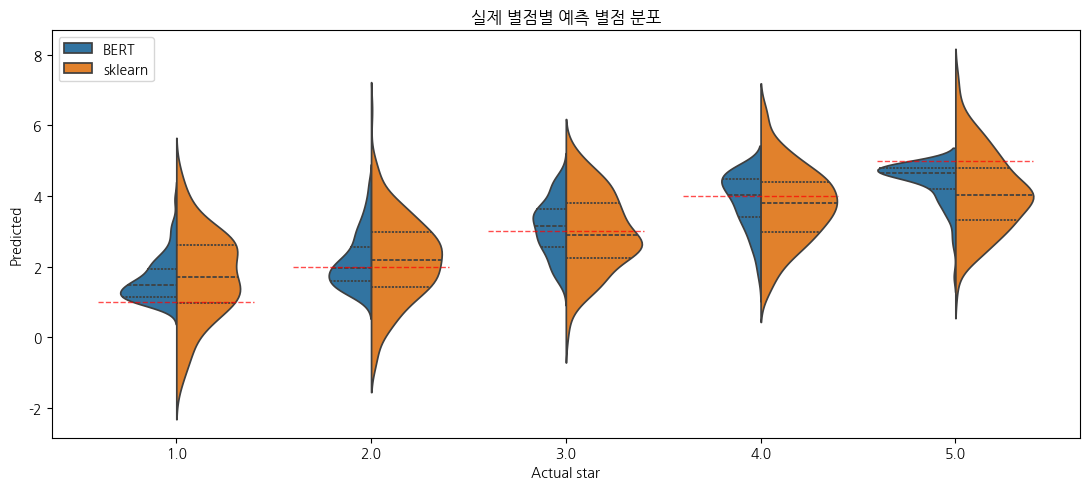
\includegraphics[width=0.92\linewidth]{assets/figures/ch09_predicted_violin.png}
\end{bookfigurelabel}



\textbf{무엇이 보이나}

\begin{itemize}
\tightlist
\item
  BERT 쪽 violin이 더 가늘고 빨간 점선 근처에 모이면 같은 actual class 안에서 예측 일관성이 높다는 뜻.
\item
  두 끝(1점, 5점)에서 분포 중심이 안쪽으로 살짝 치우치는 모양이 자주 보입니다 --- 모델이 \emph{중앙 쪽으로 회귀(regression to the mean)} 하는 경향.
\item
  sklearn 쪽 violin이 더 두텁고 길게 늘어진다면 outlier 예측이 많다는 신호.
\end{itemize}

이 그래프는 “모델이 무엇을 출력하나”의 \emph{raw 분포} 를 봅니다. 다음 그래프는 \emph{오차 자체} 에 집중합니다.



\subsection{잔차 분포}

\inlinecode{Predicted\ −\ Actual} 을 y축에 두고 0 기준선을 긋습니다. 잔차가 0 근처에 좁게 모일수록 정확하고, 양/음 한 쪽으로 치우치면 \emph{bias} 가 있다는 뜻.



\Needspace{11\baselineskip}
\begin{lstlisting}
fig, ax = plt.subplots(figsize=(11, 5))
sns.violinplot(
    data=df_compare, x="Actual star", y="Residual", hue="Model",
    split=True, inner="quart", ax=ax,
)
ax.axhline(
    0,
    color="red",
    linestyle="--",
    linewidth=1,
    alpha=0.7,
)
ax.set_title("Residual = Predicted − Actual, per actual class")
ax.set_ylabel("Residual (predicted − actual)")
ax.legend(loc="upper left")
plt.tight_layout()
\end{lstlisting}

\noindent\emph{앞뒤 블록은 모두 숫자 결과를 그림으로 확인하는 단계입니다. 길이를 나누어 같은 흐름을 단계별로 확인합니다.}

\Needspace{5\baselineskip}
\begin{lstlisting}[firstnumber=17]
plt.show()
\end{lstlisting}

\begin{bookfigurelabel}[H]{정답 별점별 잔차 분포 비교}{fig:ch09-residual-violin}
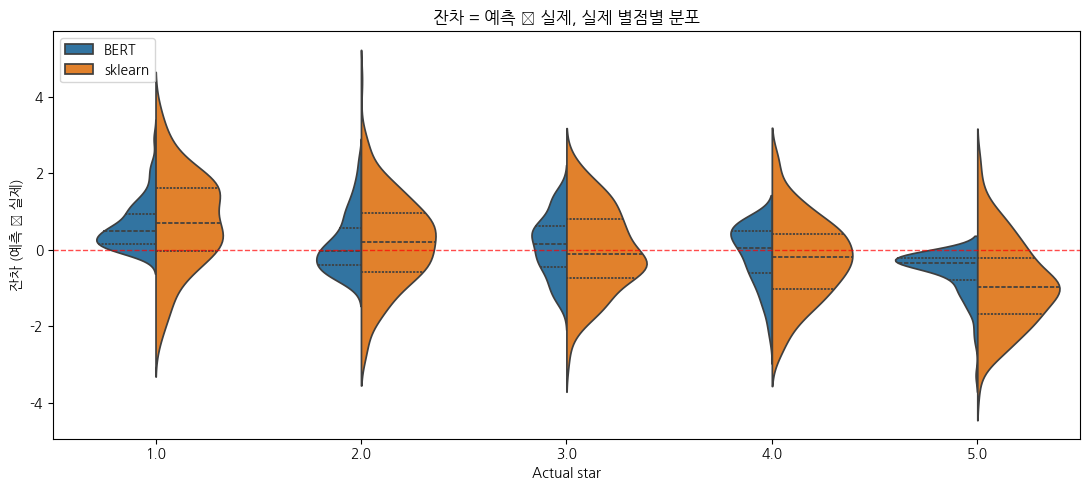
\includegraphics[width=0.92\linewidth]{assets/figures/ch09_residual_violin.png}
\end{bookfigurelabel}



\textbf{무엇이 보이나}

\begin{itemize}
\tightlist
\item
  잔차의 \emph{중심} 이 0 위/아래 어디에 있는지가 \emph{bias의 방향}. 1점 class에서 잔차 중심이 +쪽이면 모델이 “1점인데 1점보다 높게” 예측하는 경향이 있다는 뜻.
\item
  잔차의 \emph{폭} 이 그 class에서의 일반적 오차 크기. BERT가 sklearn보다 좁다면 더 정확.
\item
  두 끝 class(1점, 5점)에서 잔차 중심이 \emph{반대 방향} (1점은 +, 5점은 −)으로 치우치는 패턴이 자주 보입니다 --- 위에서 본 \emph{regression to the mean} 의 잔차 시각화 형태.
\item
  0 기준선에서 멀리 늘어진 꼬리는 큰 오차를 내는 outlier 샘플들. 어느 모델이 꼬리가 더 두꺼운지 비교.
\end{itemize}

\textbf{두 시각을 함께 보는 이유}: 시각 1은 \emph{모델이 무엇을 출력하나} (raw 분포), 시각 2는 \emph{얼마나 틀렸나} (오차 분포). 같은 데이터의 다른 시점이라 한쪽만 봐서는 놓치는 패턴이 있습니다. 정량 지표(MSE/MAE/R²) 표와 이 두 시각을 함께 읽으면 회귀 평가가 입체적이 됩니다.



\section{변형: 학습 실패 요인}

직접 다 돌리진 않고 \emph{어떤 인자를 바꾸면 무슨 일이 일어나는지} 짚습니다.

\begin{booktable}{9장 변형: 학습 실패 요인 표}{tab:ch09-05}
\begin{adjustbox}{max width=\textwidth}
\begin{tabular}{@{}ll@{}}
\toprule
바꾸는 인자 & 자주 보는 결과 \\
\midrule

\inlinecode{num\_train\_epochs=5} (더 오래) & 학습 loss는 더 줄지만 eval은 정체/악화 (overfitting) \\
\inlinecode{learning\_rate=2e-4} (10배 큼) & 학습 초반에 loss가 발산하거나 nan으로 감 \\
\inlinecode{learning\_rate=2e-7} (100배 작음) & 학습이 거의 안 됨 (loss가 안 줄어듦) \\
\inlinecode{batch\_size=4} & step 수 증가, 학습 시간 길어짐, gradient 잡음 큼 \\
\inlinecode{batch\_size=64} & T4에서 OOM 위험 (max\_length=128 + DistilBERT는 32까지가 안전) \\
\inlinecode{fp16=False} & VRAM 2배, 속도 느려짐, 결과는 비슷 \\
\inlinecode{max\_length=512} & 시퀀스 길이가 4배라 attention 비용 16배 --- T4 30분 초과 \\
\bottomrule
\end{tabular}
\end{adjustbox}
\end{booktable}

이 표가 BERT 파인튜닝의 \emph{기본 안전대} 입니다. \ref{ch:10}장 이후 모든 학습 장에서도 동일한 인자 범위에서 움직입니다.



\section{이 장에 등장한 라이브러리·함수}

\subsection{\texorpdfstring{transformers 학습 도구}{transformers 학습 도구}}

\begin{booktable}{9장 transformers 학습 도구 표}{tab:ch09-06}
\begin{adjustbox}{max width=\textwidth}
\begin{tabular}{@{}lll@{}}
\toprule
이름 & 한 줄 설명 & 다음 장에서 \\
\midrule

\inlinecode{AutoModelForSequenceClassification.from\_pretrained(...,\ num\_labels=1,\ problem\_type="regression")} & 회귀 헤드를 가진 모델 자동 구성 & \ref{ch:10}--\ref{ch:13}장에서 num\_labels·problem\_type만 바꾸어 재사용 \\
\inlinecode{Trainer} & 학습 루프 + 평가 + 로깅 + 체크포인트 자동화 & 모든 Phase 1·2 학습 장의 기본 \\
\inlinecode{TrainingArguments} & 학습 하이퍼파라미터 묶음 & num\_epochs / batch / lr / fp16 등 인자 동일 \\
\inlinecode{Trainer.train()}, \inlinecode{.evaluate()}, \inlinecode{.predict()} & 학습 / 평가 / 추론 호출 & 모든 학습 장 \\
\bottomrule
\end{tabular}
\end{adjustbox}
\end{booktable}

\subsection{Trainer의 역할}

\begin{itemize}
\tightlist
\item
  \textbf{DataCollatorWithPadding} 생성 (\inlinecode{tokenizer} 인자 보고)
\item
  학습 루프 (epoch 반복, batch 단위 forward/backward/optimizer step)
\item
  평가 (\inlinecode{eval\_strategy} 에 따라)
\item
  fp16 mixed precision (\inlinecode{fp16=True} 옵션 보고)
\item
  로깅 (\inlinecode{logging\_steps})
\item
  체크포인트 (\inlinecode{save\_strategy})
\item
  gradient clipping (기본 1.0)
\item
  learning rate scheduler (기본 linear warmup → linear decay)
\end{itemize}

\subsection{\texorpdfstring{compute\_metrics}{compute\_metrics 함수 시그니처}}

\Needspace{5\baselineskip}
\begin{lstlisting}
def compute_metrics(eval_pred) -> dict:
    preds, labels = eval_pred       # numpy arrays
    return {"metric_name": value, ...}
\end{lstlisting}



\section{체크포인트 질문}

\begin{enumerate}
\def\labelenumi{\arabic{enumi}.}
\tightlist
\item
  \inlinecode{num\_labels=1} 과 \inlinecode{problem\_type="regression"} 두 인자가 \inlinecode{Trainer} 동작에 어떤 영향을 주나요?
\item
  학습 중 VRAM이 모델 가중치만 있는 상태보다 더 큰 이유는 무엇인가요? (옵티마이저·gradient·activation)
\item
  sklearn \inlinecode{LinearRegression} 의 정규방정식과 BERT의 Adam optimizer는 같은 MSE를 최소화하는데도 학습 시간·결정성이 왜 그렇게 다른가요?
\item
  \inlinecode{compute\_metrics} 함수의 입력 \inlinecode{eval\_pred} 는 어떤 형태인가요? 회귀와 분류에서 어떻게 달라지나요?
\end{enumerate}



\section{FAQ}

\begin{faqBox}{Q1. (실무) 학습 중 loss가 nan이 됩니다. 어떻게 하나요?}

가장 흔한 원인이 fp16 수치 오버플로우입니다. 해결 순서:

\begin{enumerate}
\def\labelenumi{\arabic{enumi}.}
\tightlist
\item
  \inlinecode{fp16=False} 로 두고 다시 시도. nan이 사라지면 fp16이 원인.
\item
  학습률을 낮춥니다 (\inlinecode{learning\_rate=1e-5} 또는 \inlinecode{5e-6}).
\item
  그래도 안 되면 \inlinecode{gradient\_clipping} 을 더 작게 (\inlinecode{max\_grad\_norm=0.5}).
\item
  입력 데이터에 비정상값(빈 문자열, 너무 긴 시퀀스)이 있는지 확인.
\end{enumerate}

T4는 fp16만 지원하고 bf16이 안 됩니다. fp16이 자주 nan을 일으키면 fp32로 가는 게 가장 안전한 fallback입니다.

\end{faqBox}

\begin{faqBox}{Q2. (실무) \inlinecode{Trainer.train()} 한 줄로 GPU 사용률이 낮은데 어떻게 올리나요?}

세 가지 흔한 원인.

\begin{enumerate}
\def\labelenumi{\arabic{enumi}.}
\tightlist
\item
  \textbf{batch\_size가 작음}: T4에서 DistilBERT는 max\_length=128, batch\_size=32까지 무난. \inlinecode{per\_device\_train\_batch\_size} 를 키워보세요.
\item
  \textbf{DataLoader 워커 부족}: \inlinecode{dataloader\_num\_workers=2} 또는 4로 늘려 CPU에서 토크나이저 처리가 GPU를 기다리지 않게.
\item
  \textbf{\inlinecode{fp16=True} 로 메모리 여유 확보}: 같은 VRAM에 더 큰 batch를 담을 수 있음.
\end{enumerate}

\Needspace{8\baselineskip}
\begin{lstlisting}
training_args = TrainingArguments(
    ...,
    per_device_train_batch_size=32,
    fp16=True,
    dataloader_num_workers=2,
)
\end{lstlisting}

\end{faqBox}

\begin{faqBox}{Q3. (실무) 학습 중간에 끊겼는데 이어서 학습하려면?}

\inlinecode{save\_strategy="epoch"} 으로 체크포인트를 저장해 두면 다음과 같이 이어 학습할 수 있습니다.

\Needspace{5\baselineskip}
\begin{lstlisting}
trainer.train(resume_from_checkpoint="./output/checkpoint-500")

trainer.train(resume_from_checkpoint=True)
\end{lstlisting}

이 장는 학습이 짧아 \inlinecode{save\_strategy="no"} 로 두었습니다. \ref{ch:14}장 같은 긴 학습이나 실무 프로젝트에선 \inlinecode{save\_strategy="epoch"} + \inlinecode{save\_total\_limit=2} 가 표준 패턴입니다.

\end{faqBox}

\begin{faqBox}{Q4. (이론) BERT의 \texttt{{[}CLS{]}} 토큰이 회귀 출력을 어떻게 만들어내나요?}

DistilBERT의 마지막 layer hidden state는 shape \inlinecode{(batch,\ seq\_len,\ 768)} 입니다. 분류·회귀 헤드는 그중 \emph{첫 번째 토큰} 의 hidden state(\texttt{{[}CLS{]}} 위치)를 가져와 \inlinecode{Linear(768,\ num\_labels)} 에 통과시킵니다.

\Needspace{10\baselineskip}
\begin{lstlisting}
hidden_states = self.distilbert(input_ids).last_hidden_state
# (B, L, 768)
cls_hidden = hidden_states[:, 0]                              # (
    B,
    768,
)
logits = self.classifier(cls_hidden)
# (B, num_labels)
\end{lstlisting}

\texttt{{[}CLS{]}} 위치의 hidden state는 사전학습 단계부터 \emph{전체 문장의 의미를 모으는 자리} 로 학습됐습니다 (attention을 통해). 그래서 분류·회귀 헤드를 \texttt{{[}CLS{]}} 위치에 붙이는 게 자연스럽고, BERT 표준 관행이 됐습니다.

\end{faqBox}

\begin{faqBox}{Q5. (이론) 사전학습된 BERT를 가져다 쓰는 게 sklearn보다 왜 더 잘 되나요?}

세 가지 이유.

\begin{enumerate}
\def\labelenumi{\arabic{enumi}.}
\tightlist
\item
  \textbf{단어 독립 가정 탈피}: TF-IDF는 \inlinecode{"not\ bad"} 와 \inlinecode{"bad"} 를 구분 못 합니다. BERT는 attention으로 \inlinecode{"not"} 과 \inlinecode{"bad"} 의 \emph{조합} 을 학습합니다.
\item
  \textbf{사전학습으로 얻은 일반 지식}: 위키피디아·BookCorpus로 학습한 단어 의미·문법·상식이 본체에 인코딩돼 있고, 우리는 그 위에 task-specific 헤드만 미세 조정.
\item
  \textbf{분포 표현(distributed representation)}: 768차원 hidden state로 단어·문장을 벡터로 표현하니 미묘한 의미 차이도 거리로 잡힘.
\end{enumerate}

다만 \emph{모든} 데이터에서 BERT가 sklearn을 압도하는 건 아닙니다. Yelp 별점은 단어 빈도가 강한 신호라 sklearn도 꽤 잘하고, 데이터가 작거나(수백 건) feature가 명확한 task(분야 키워드 분류)는 sklearn이 BERT보다 빠르고 가성비 좋습니다.

\end{faqBox}

\begin{faqBox}{Q6. (실무) \inlinecode{output\_dir} 에 뭐가 저장되나요?}

\inlinecode{save\_strategy} 가 \inlinecode{"no"} 가 아니면:

\begin{itemize}
\tightlist
\item
  \texttt{checkpoint-\{step\}/} --- 모델 가중치, 옵티마이저 상태, scheduler 상태, RNG state (재현 가능한 재개)
\item
  \inlinecode{pytorch\_model.bin} 또는 \inlinecode{model.safetensors} --- 모델 가중치
\item
  \inlinecode{config.json} --- 모델 config (\ref{ch:07}장 부록 참고)
\item
  \inlinecode{tokenizer.json}, \inlinecode{vocab.txt} 등 --- 토크나이저 (\inlinecode{tokenizer=...} 인자가 있을 때)
\item
  \inlinecode{training\_args.bin} --- 학습 인자 dump
\item
  \inlinecode{trainer\_state.json} --- loss/metric 로그
\end{itemize}

Colab에서 \inlinecode{output\_dir} 를 Drive 경로로 잡으면 세션이 끊겨도 보존됩니다 (\inlinecode{output\_dir="/content/drive/MyDrive/runs/ch09"}).
\end{faqBox}



\section{오류 실험 (선택)}

다음 코드를 돌려보고 어떤 에러가 나는지 보세요.

\Needspace{11\baselineskip}
\begin{lstlisting}
def tokenize_int(batch):
    out = tokenizer(
        batch["text"],
        truncation=True,
        max_length=128,
    )
    out["labels"] = batch["label"]
    return out

train_int = train_ds.select(range(100)).map(tokenize_int, batched=True).remove_columns(["text", "label"])
\end{lstlisting}

힌트: 회귀 task에서 라벨이 int면 \inlinecode{MSELoss} 가 squared error 계산은 하지만 dtype 경고나 미묘한 문제가 생길 수 있습니다. \inlinecode{problem\_type="regression"} 은 라벨이 \emph{float} 이라고 가정합니다. \inlinecode{label2id}/\inlinecode{id2label} 도 자동 안 만들어집니다.

회귀 라벨은 \emph{항상 float} 으로 변환하는 게 안전합니다.



\begin{previewBox}{미리보기: 다음 장}

\textbf{\ref{ch:10}장. BERT 이진 분류 A (Sigmoid \& BCE)}

\begin{itemize}
\tightlist
\item
  \ref{ch:04}장 (sklearn) 에서 본 동등성의 BERT 버전 시작
\item
  \inlinecode{num\_labels=1}, sigmoid, \inlinecode{BCEWithLogitsLoss} 로 Yelp 이진화 학습
\item
  \ref{ch:09}장의 \inlinecode{Trainer} 골격을 그대로 재사용
\end{itemize}

\textbf{\ref{ch:11}장. BERT 이진 분류 B (Softmax \& CE)} 가 그 다음에 이어집니다 (BERT 표준). 두 장의 \inlinecode{predict\_proba} 가 거의 일치하는지 비교가 핵심.
\end{previewBox}
